\begin{pastexam}[label={px:ncku-108-prog-03}]{成大資訊聯招 108 學年度 第 3 題}
（問答）

Given the following 8 runs: (20\%)
\begin{center}
\setlength{\tabcolsep}{3pt}
\begin{tabular}{|c|c|c|c|c|c|c|c|c|c|c|c|c|c|c|}
\cline{1-1}\cline{3-3}\cline{5-5}\cline{7-7}\cline{9-9}\cline{11-11}\cline{13-13}\cline{15-15}
5 & \multicolumn{1}{c|}{} & 8 & \multicolumn{1}{c|}{} & 23 & \multicolumn{1}{c|}{} & 1 & \multicolumn{1}{c|}{} & 4 & \multicolumn{1}{c|}{} & 3 & \multicolumn{1}{c|}{} & 16 & \multicolumn{1}{c|}{} & 11 \\
\cline{1-1}\cline{3-3}\cline{5-5}\cline{7-7}\cline{9-9}\cline{11-11}\cline{13-13}\cline{15-15}
13 & \multicolumn{1}{c|}{} & 18 & \multicolumn{1}{c|}{} & 27 & \multicolumn{1}{c|}{} & 15 & \multicolumn{1}{c|}{} & 10 & \multicolumn{1}{c|}{} & 20 & \multicolumn{1}{c|}{} & 17 & \multicolumn{1}{c|}{} & 21 \\
\cline{1-1}\cline{3-3}\cline{5-5}\cline{7-7}\cline{9-9}\cline{11-11}\cline{13-13}\cline{15-15}
22 & \multicolumn{1}{c|}{} & 30 & \multicolumn{1}{c|}{} & 38 & \multicolumn{1}{c|}{} & 19 & \multicolumn{1}{c|}{} & 24 & \multicolumn{1}{c|}{} & 32 & \multicolumn{1}{c|}{} & 35 & \multicolumn{1}{c|}{} & 25 \\
\cline{1-1}\cline{3-3}\cline{5-5}\cline{7-7}\cline{9-9}\cline{11-11}\cline{13-13}\cline{15-15}
\end{tabular}
\end{center}
\begin{enumerate}[label=(\arabic*)]
\item Draw the corresponding winner tree. (5\%)
\item Draw the restructured winner tree after one record has been output. (5\%)
\item Draw the loser tree based on the answer of question (2). (5\%)
\item Derive the total required time to merge $n$ records through a winner tree with $k$ runs. (5\%)
\end{enumerate}
\end{pastexam}

\begin{pastsoln}
約定：照資結書第~15.3~節。 八個串由左到右叫 $R_1, \ldots, R_8$，每個串目前最前
面的鍵是一位選手，鍵小的贏（本題的鍵都不同，不會平手）。 節點編號和堆積一樣：內部節點
$1$ 到 $7$，葉節點 $8$ 到 $15$，葉節點 $7 + i$ 代表 $R_i$。 圖中內部節點寫鍵，旁邊小字是來
自哪個串；葉節點下面的小字是那個串還沒讀的部分。

\begin{center}
\begin{tabular}{l}
$R_1 = \langle 5, 13, 22 \rangle$, $R_2 = \langle 8, 18, 30 \rangle$, $R_3 = \langle 23, 27, 38 \rangle$, $R_4 = \langle 1, 15, 19 \rangle$, \\
$R_5 = \langle 4, 10, 24 \rangle$, $R_6 = \langle 3, 20, 32 \rangle$, $R_7 = \langle 16, 17, 35 \rangle$, $R_8 = \langle 11, 21, 25 \rangle$.
\end{tabular}
\end{center}

(1) 由下往上比賽：節點 4 是 $5$ 對 $8$，$5$（$R_1$）贏；節點 5 是 $23$ 對 $1$，$1$（$R_4$）贏；節點 6
是 $4$ 對 $3$，$3$（$R_6$）贏；節點 7 是 $16$ 對 $11$，$11$（$R_8$）贏。 節點 2 是 $5$ 對 $1$，
$1$ 贏；節點 3 是 $3$ 對 $11$，$3$ 贏；節點 1 是 $1$ 對 $3$，冠軍是 $1$（$R_4$）。 共比 $7$ 次。

\begin{center}
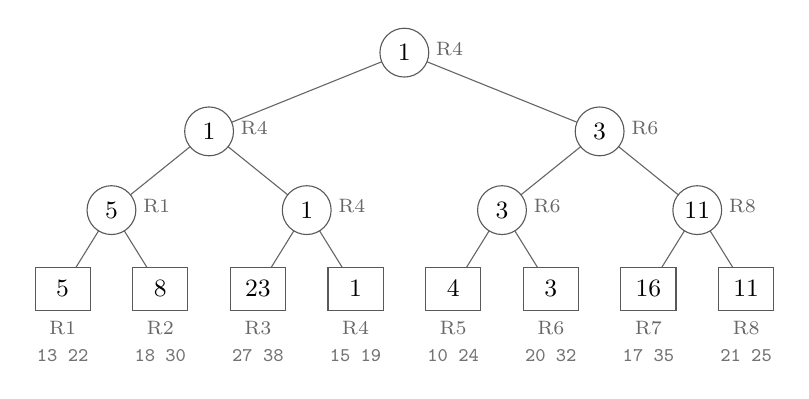
\begin{tikzpicture}[x=0.62cm,y=1.00cm,
    lte/.style={draw=black!60},
    ltn/.style={circle, draw=black!65, minimum size=0.62cm, inner sep=0pt, font=\small},
    ltchg/.style={draw=memStroke, very thick, fill=memFill},
    ltwin/.style={rectangle, draw=coreStroke, thick, fill=coreFill, minimum width=0.7cm, minimum height=0.55cm, font=\small},
    ltleaf/.style={rectangle, draw=black!65, minimum width=0.7cm, minimum height=0.55cm, font=\small},
    ltnew/.style={draw=greenStroke, very thick, fill=greenFill},
    rlab/.style={font=\scriptsize, text=black!60, inner sep=1pt},
    restlab/.style={font=\scriptsize\ttfamily, text=black!55}]
\draw[lte] (7,-1) -- (3,-2);
\draw[lte] (7,-1) -- (11,-2);
\draw[lte] (3,-2) -- (1,-3);
\draw[lte] (3,-2) -- (5,-3);
\draw[lte] (11,-2) -- (9,-3);
\draw[lte] (11,-2) -- (13,-3);
\draw[lte] (1,-3) -- (0,-4);
\draw[lte] (1,-3) -- (2,-4);
\draw[lte] (5,-3) -- (4,-4);
\draw[lte] (5,-3) -- (6,-4);
\draw[lte] (9,-3) -- (8,-4);
\draw[lte] (9,-3) -- (10,-4);
\draw[lte] (13,-3) -- (12,-4);
\draw[lte] (13,-3) -- (14,-4);
\node[ltn, fill=white] at (7,-1) {$1$};
\node[rlab, anchor=west] at (7.58,-0.95) {R4};
\node[ltn, fill=white] at (3,-2) {$1$};
\node[rlab, anchor=west] at (3.58,-1.95) {R4};
\node[ltn, fill=white] at (11,-2) {$3$};
\node[rlab, anchor=west] at (11.58,-1.95) {R6};
\node[ltn, fill=white] at (1,-3) {$5$};
\node[rlab, anchor=west] at (1.58,-2.95) {R1};
\node[ltn, fill=white] at (5,-3) {$1$};
\node[rlab, anchor=west] at (5.58,-2.95) {R4};
\node[ltn, fill=white] at (9,-3) {$3$};
\node[rlab, anchor=west] at (9.58,-2.95) {R6};
\node[ltn, fill=white] at (13,-3) {$11$};
\node[rlab, anchor=west] at (13.58,-2.95) {R8};
\node[ltleaf, fill=white] at (0,-4) {$5$};
\node[rlab] at (0,-4.5) {R1};
\node[restlab] at (0,-4.85) {13 22};
\node[ltleaf, fill=white] at (2,-4) {$8$};
\node[rlab] at (2,-4.5) {R2};
\node[restlab] at (2,-4.85) {18 30};
\node[ltleaf, fill=white] at (4,-4) {$23$};
\node[rlab] at (4,-4.5) {R3};
\node[restlab] at (4,-4.85) {27 38};
\node[ltleaf, fill=white] at (6,-4) {$1$};
\node[rlab] at (6,-4.5) {R4};
\node[restlab] at (6,-4.85) {15 19};
\node[ltleaf, fill=white] at (8,-4) {$4$};
\node[rlab] at (8,-4.5) {R5};
\node[restlab] at (8,-4.85) {10 24};
\node[ltleaf, fill=white] at (10,-4) {$3$};
\node[rlab] at (10,-4.5) {R6};
\node[restlab] at (10,-4.85) {20 32};
\node[ltleaf, fill=white] at (12,-4) {$16$};
\node[rlab] at (12,-4.5) {R7};
\node[restlab] at (12,-4.85) {17 35};
\node[ltleaf, fill=white] at (14,-4) {$11$};
\node[rlab] at (14,-4.5) {R8};
\node[restlab] at (14,-4.85) {21 25};
\end{tikzpicture}
\end{center}

(2) 輸出冠軍 $1$，$R_4$ 補上下一個鍵 $15$，沿著 $R_4$ 的葉節點（節點 11）往上重賽，每一層和兄弟節點的贏
家比一次：節點 5 是 $15$ 對兄弟 $R_3$ 的 $23$，$15$ 贏；節點 2 是 $15$ 對兄弟節點 4 的贏家 $5$，
$5$（$R_1$）贏；節點 1 是 $5$ 對兄弟節點 3 的贏家 $3$，$3$（$R_6$）贏。 新的冠軍是 $3$，下一
個輸出的就是它。 只比了 $3 = \lg 8$ 次。 橘色是重賽過的節點，綠色是剛補上新鍵的葉節點。

\begin{center}
\begin{tikzpicture}[x=0.62cm,y=1.00cm,
    lte/.style={draw=black!60},
    ltn/.style={circle, draw=black!65, minimum size=0.62cm, inner sep=0pt, font=\small},
    ltchg/.style={draw=memStroke, very thick, fill=memFill},
    ltwin/.style={rectangle, draw=coreStroke, thick, fill=coreFill, minimum width=0.7cm, minimum height=0.55cm, font=\small},
    ltleaf/.style={rectangle, draw=black!65, minimum width=0.7cm, minimum height=0.55cm, font=\small},
    ltnew/.style={draw=greenStroke, very thick, fill=greenFill},
    rlab/.style={font=\scriptsize, text=black!60, inner sep=1pt},
    restlab/.style={font=\scriptsize\ttfamily, text=black!55}]
\draw[lte] (7,-1) -- (3,-2);
\draw[lte] (7,-1) -- (11,-2);
\draw[lte] (3,-2) -- (1,-3);
\draw[lte] (3,-2) -- (5,-3);
\draw[lte] (11,-2) -- (9,-3);
\draw[lte] (11,-2) -- (13,-3);
\draw[lte] (1,-3) -- (0,-4);
\draw[lte] (1,-3) -- (2,-4);
\draw[lte] (5,-3) -- (4,-4);
\draw[lte] (5,-3) -- (6,-4);
\draw[lte] (9,-3) -- (8,-4);
\draw[lte] (9,-3) -- (10,-4);
\draw[lte] (13,-3) -- (12,-4);
\draw[lte] (13,-3) -- (14,-4);
\node[ltn, fill=white, ltchg] at (7,-1) {$3$};
\node[rlab, anchor=west] at (7.58,-0.95) {R6};
\node[ltn, fill=white, ltchg] at (3,-2) {$5$};
\node[rlab, anchor=west] at (3.58,-1.95) {R1};
\node[ltn, fill=white] at (11,-2) {$3$};
\node[rlab, anchor=west] at (11.58,-1.95) {R6};
\node[ltn, fill=white] at (1,-3) {$5$};
\node[rlab, anchor=west] at (1.58,-2.95) {R1};
\node[ltn, fill=white, ltchg] at (5,-3) {$15$};
\node[rlab, anchor=west] at (5.58,-2.95) {R4};
\node[ltn, fill=white] at (9,-3) {$3$};
\node[rlab, anchor=west] at (9.58,-2.95) {R6};
\node[ltn, fill=white] at (13,-3) {$11$};
\node[rlab, anchor=west] at (13.58,-2.95) {R8};
\node[ltleaf, fill=white] at (0,-4) {$5$};
\node[rlab] at (0,-4.5) {R1};
\node[restlab] at (0,-4.85) {13 22};
\node[ltleaf, fill=white] at (2,-4) {$8$};
\node[rlab] at (2,-4.5) {R2};
\node[restlab] at (2,-4.85) {18 30};
\node[ltleaf, fill=white] at (4,-4) {$23$};
\node[rlab] at (4,-4.5) {R3};
\node[restlab] at (4,-4.85) {27 38};
\node[ltleaf, fill=white, ltnew] at (6,-4) {$15$};
\node[rlab] at (6,-4.5) {R4};
\node[restlab] at (6,-4.85) {19};
\node[ltleaf, fill=white] at (8,-4) {$4$};
\node[rlab] at (8,-4.5) {R5};
\node[restlab] at (8,-4.85) {10 24};
\node[ltleaf, fill=white] at (10,-4) {$3$};
\node[rlab] at (10,-4.5) {R6};
\node[restlab] at (10,-4.85) {20 32};
\node[ltleaf, fill=white] at (12,-4) {$16$};
\node[rlab] at (12,-4.5) {R7};
\node[restlab] at (12,-4.85) {17 35};
\node[ltleaf, fill=white] at (14,-4) {$11$};
\node[rlab] at (14,-4.5) {R8};
\node[restlab] at (14,-4.85) {21 25};
\end{tikzpicture}
\end{center}

(3) 敗者樹的每個內部節點記那場比賽的\textbf{輸家}，另外用節點 $0$ 記冠軍（資結書第~15.3.4~節）。
(2) 的狀態下每一場比賽的兩方和勝負都已經知道，把輸家記下來就是：節點 4 記 $8$（$R_2$），節點 5
記 $23$（$R_3$），節點 6 記 $4$（$R_5$），節點 7 記 $16$（$R_7$），節點 2 記 $15$（$R_4$），節
點 3 記 $11$（$R_8$），節點 1 記 $5$（$R_1$），節點 0 記冠軍 $3$（$R_6$）。

\begin{center}
\begin{tikzpicture}[x=0.62cm,y=1.00cm,
    lte/.style={draw=black!60},
    ltn/.style={circle, draw=black!65, minimum size=0.62cm, inner sep=0pt, font=\small},
    ltchg/.style={draw=memStroke, very thick, fill=memFill},
    ltwin/.style={rectangle, draw=coreStroke, thick, fill=coreFill, minimum width=0.7cm, minimum height=0.55cm, font=\small},
    ltleaf/.style={rectangle, draw=black!65, minimum width=0.7cm, minimum height=0.55cm, font=\small},
    ltnew/.style={draw=greenStroke, very thick, fill=greenFill},
    rlab/.style={font=\scriptsize, text=black!60, inner sep=1pt},
    restlab/.style={font=\scriptsize\ttfamily, text=black!55}]
\draw[lte] (7,-1) -- (3,-2);
\draw[lte] (7,-1) -- (11,-2);
\draw[lte] (3,-2) -- (1,-3);
\draw[lte] (3,-2) -- (5,-3);
\draw[lte] (11,-2) -- (9,-3);
\draw[lte] (11,-2) -- (13,-3);
\draw[lte] (1,-3) -- (0,-4);
\draw[lte] (1,-3) -- (2,-4);
\draw[lte] (5,-3) -- (4,-4);
\draw[lte] (5,-3) -- (6,-4);
\draw[lte] (9,-3) -- (8,-4);
\draw[lte] (9,-3) -- (10,-4);
\draw[lte] (13,-3) -- (12,-4);
\draw[lte] (13,-3) -- (14,-4);
\draw[lte] (7,-1) -- (7,0);
\node[ltwin] at (7,0) {$3$};
\node[rlab, anchor=west] at (7.58,0) {R6};
\node[ltn, fill=white] at (7,-1) {$5$};
\node[rlab, anchor=west] at (7.58,-0.95) {R1};
\node[ltn, fill=white] at (3,-2) {$15$};
\node[rlab, anchor=west] at (3.58,-1.95) {R4};
\node[ltn, fill=white] at (11,-2) {$11$};
\node[rlab, anchor=west] at (11.58,-1.95) {R8};
\node[ltn, fill=white] at (1,-3) {$8$};
\node[rlab, anchor=west] at (1.58,-2.95) {R2};
\node[ltn, fill=white] at (5,-3) {$23$};
\node[rlab, anchor=west] at (5.58,-2.95) {R3};
\node[ltn, fill=white] at (9,-3) {$4$};
\node[rlab, anchor=west] at (9.58,-2.95) {R5};
\node[ltn, fill=white] at (13,-3) {$16$};
\node[rlab, anchor=west] at (13.58,-2.95) {R7};
\node[ltleaf, fill=white] at (0,-4) {$5$};
\node[rlab] at (0,-4.5) {R1};
\node[restlab] at (0,-4.85) {13 22};
\node[ltleaf, fill=white] at (2,-4) {$8$};
\node[rlab] at (2,-4.5) {R2};
\node[restlab] at (2,-4.85) {18 30};
\node[ltleaf, fill=white] at (4,-4) {$23$};
\node[rlab] at (4,-4.5) {R3};
\node[restlab] at (4,-4.85) {27 38};
\node[ltleaf, fill=white] at (6,-4) {$15$};
\node[rlab] at (6,-4.5) {R4};
\node[restlab] at (6,-4.85) {19};
\node[ltleaf, fill=white] at (8,-4) {$4$};
\node[rlab] at (8,-4.5) {R5};
\node[restlab] at (8,-4.85) {10 24};
\node[ltleaf, fill=white] at (10,-4) {$3$};
\node[rlab] at (10,-4.5) {R6};
\node[restlab] at (10,-4.85) {20 32};
\node[ltleaf, fill=white] at (12,-4) {$16$};
\node[rlab] at (12,-4.5) {R7};
\node[restlab] at (12,-4.85) {17 35};
\node[ltleaf, fill=white] at (14,-4) {$11$};
\node[rlab] at (14,-4.5) {R8};
\node[restlab] at (14,-4.85) {21 25};
\end{tikzpicture}
\end{center}

檢查：從 (1) 的狀態建敗者樹，再對 $R_4$ 做一次 \proc{Adjust}（資結書虛擬碼~15.5），結
果也是這棵樹：$15$ 在節點 5 贏了記在那裡的 $23$（$23$ 留下），在節點 2 輸給記在那裡的 $5$
（$15$ 留下、$5$ 往上），往上走的 $5$ 在節點 1 輸給記在那裡的 $3$（$5$ 留下、$3$ 往上），冠軍 $3$ 放進節點 0。

(4) 設 $k$ 個串總共有 $n$ 筆紀錄，每個串至少一筆，所以 $k \le n$。
\begin{itemize}
\item 建勝者樹：$k - 1$ 個內部節點各比一場，$O(k)$。
\item 每輸出一筆：冠軍的串補上下一個鍵（讀完了補 $\infty$），從它的葉節點往上到根重賽。 有
$k$ 個葉節點的完整二元樹，葉節點的深度不超過 $\lceil \lg k \rceil$，所以最多重賽
$\lceil \lg k \rceil$ 層，每層比一次、做常數的工作，$O(\lg k)$。
\item 一共輸出 $n$ 筆，$n \cdot O(\lg k)$。
\end{itemize}
總時間 $O(k) + O(n \lg k) = O(n \lg k)$（$k \le n$）。 和直接每次掃 $k$ 個串的最前面相比
（每筆 $k - 1$ 次比較，總共 $O(nk)$），$k$ 大時省很多。 若問的是外部排序的一趟合併，還要
加上讀寫區塊的時間，見資結書第~15.3.2~節。
\end{pastsoln}
